\section{Durchführung}
\label{sec:Durchführung}

Der grundlegende Aufbau des Versuchs ist in Abbildung \ref{fig:aufbau} dargestellt.
Als Quelle dient dabei ein 241-Americium Präparat. Die ausgehende Alphastrahlung
wird beim Durchlaufen des Kollimators in Richtung der Folie gebündelt, an welcher
sie letztendlich gestreut wird. Der dahinter liegende Detektor ist auf einer Schiene
um die Folie beweglich, wodurch die unter verschiedenen Winkeln gestreute Strahlung
gemessen werden kann. Bei dem Detektor handelt es sich um einen Surface-Barrier-Detektor.
Dieser funktioniert im Prinzip wie eine in Sperrrichtung betriebene Diode. In einer durch einen p-n-Übergang
entstehenden Verarmungszone erzeugt einfallende Strahlung Elektronen-Loch-Paare,
welche einen messbaren elektrischen Impuls erzeugen. Dieser Impuls kann mittels eines
Verstärkers dann noch verstärkt werden.

Der gesamte Aufbau befindet sich wiederum in einer Vakuumapparatur, da sich ab einem
Kammerdruck von etwa $\SI{200}{\milli\bar}$ bereits Energieverluste durch das Bremsvermögen
der $\alpha$-Teilchen in Luft bemerkbar machen. 
Die Apparatur kann durch eine Drehschieberpumpe evakuiert werden. Die Pumpe besteht im Wesentlichen
aus einem Hohlzylinder, in dem ein weiterer Zylinder rotiert. Der rotierende Zylinder
befindet sich jedoch nicht mittig in dem Hohlzylinder, sondern berührt dessen Innenwand
zwischen Ein- und Auslassöffnung der Luft. Des Weiteren sind an diesem sogenannte
Drehschieber angebracht, welche durch eine Feder gegen die Innenwand gedrückt werden.
So wird das Hohlzylindervolumen in drei Bereiche unterteilt und durch Rotation des
inneren Zylinders entsprechend Luft angesaugt und abgepumpt.

\begin{figure}[H]
  \centering
  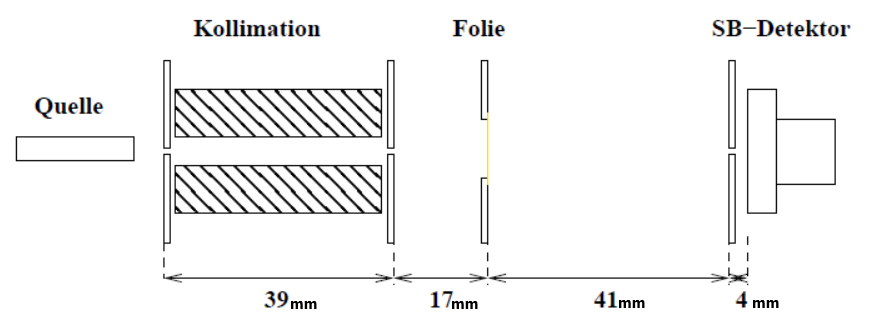
\includegraphics[height=6cm]{Aufbau.PNG}
  \caption{Schematischer Aufbau des Versuchs. \cite{sample1}}
  \label{fig:aufbau}
\end{figure}

Im ersten Versuchsteil befindet sich noch keine Folie zwischen Quelle und Detektor
Es werden bei evakuiertem Volumen die am Detektor sowie auch am Verstärker
abgegriffenen  Spannungsimpulse auf einem Oszilloskop sichtbar gemacht und die
entstehenden Bilder gespeichert. Der Detektor befindet sich dabei bei null Grad Auslenkung.

Anschließend wird die Höhe der verstärkten Impulse bei unterschiedlichem Druck
in der Vakuumapparatur gemessen (Bereich 0-200 mbar). Die gleiche Messung wird auch
noch einmal mit einer eingefügten Goldfolie ($\SI{2}{\micro\meter}$) wiederholt.

Sodann wird das Volumen wieder vollständig evakuiert. Nun werden
mithilfe des beweglichen Detektors die Zählraten unter verschiedenen Winkeln gemessen.

Zuletzt werden dann noch einmal die Zählraten unter einem bestimmten Winkel für
drei weitere Folien ($\SI{4}{\micro\meter}$ Goldfolie, $\SI{3}{\micro\meter}$ Aluminiumfolie,
$\SI{1}{\micro\meter}$ Bismutfolie) ermittelt.
